\chapter{Новые встречи со старыми знакомыми}

\setlength{\epigraphwidth}{.53\textwidth}
\epigraph{Забыть ли дружбу прежних дней\\
И не грустить о ней?}{--- Роберт Бёрнс (1759---1796)}

Как и вино, головоломки могут улучшаться с возрастом, приобретая новые, захватывающие версии, а иногда и лучшие решения.
В этой главе представлены головоломки, которые знакомы многим.
Однако даже если вы очень хорошо знаете какие-то из них, 
вы обнаружите новые удивительные повороты!

Один из самых запоминающихся персонажей головоломок --- логик, любящий отдыхать на южных морях.
Если верить Мартину Гарднеру \cite{27}, этот логик постоянно теряется и вынужден спрашивать аборигенов дорогу.

\subsection*{Три аборигена на перекрёстке}

Гарднеровский логик снова поехал на юг и, как обычно, стоит на развилке, желая узнать, по какой из двух дорог можно добраться до деревни.
На этот раз рядом с ним три аборигена, по одному из трёх племён:
племени правдолюбов,
племени лжецов
и племени случайно отвечающих.
Конечно же, логик не знает, к какому племени отнести каждого из аборигенов.
Ему разрешается задать только два вопроса с ответом «да» или «нет».
Каждый вопрос задаётся только одному аборигену.
Сможет ли он получить необходимую информацию?
А что если ему разрешено задать только \emph{один} вопрос с ответом «да» или «нет»?

\medskip

Перейдём к известной и изящной геометрической головоломке, которая, к моему стыду, появилась в моей предыдущей книге \cite{59} с не вполне верным решением.

\subsection*{Новая встреча с тремя окружностями}

Назовём фокусом двух окружностей пересечение двух их общих внешних касательных.
Таким образом, если три окружности имеют разные радиусы (и ни одна не лежит в другой), то они определяют три фокуса (см. рис. \ref{pic:3circ}).
Докажите, что эти три фокуса лежат на одной прямой.

\begin{figure}[h!]
\centering
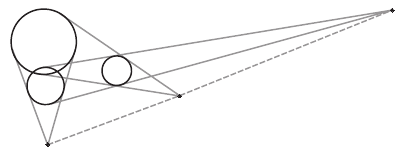
\includegraphics[scale=1]{pics/3circs}
\caption{Три окружности и их фокусы.}
\label{pic:3circ}
\end{figure}

\parit{Примечания.}
В моей предыдущей книге \cite{59} предлагается построить три сферы с экваторами на данных окружностях, а затем рассмотреть плоскость, касающуюся этих трёх сфер.
Однако Джером Льюис, профессор информатики в Университете Южной Каролины в Апстейте, справедливо указал мне на то, что такой плоскости может не быть!
Например, её нет, когда две окружности большие, и между ними находится меньшая.

Однако доказательство можно спасти, не отказываясь от основной идеи.
Попробуйте найти способ.

\medskip

Следующая задача является отличным представителем головоломок про знания о знаниях.

\subsection*{Самоубийцы Точкинска}

У каждого жителя Точкинска есть красная или синяя точка на лбу.
Если он когда-либо решит, что знает, какого цвета его точка, то покончит с собой.
Все точкинцы встречаются каждый день и видят друг друга.
Однажды приезжий сказал им что-то (что угодно не тривиальное) о числе синих точек.
Докажите, что рано или поздно все точкинцы покончат с собой.

\parit{Примечания.} Что-то \emph{нетривиальное} означает, что некоторое число синих точек делает это утверждение верным, а какое-то другое число --- неверным.
Однако мы не предполагаем, что то, что сказал им приезжий, является правдой!
Увы, точкинцы легковерны --- они верят всему, что слышат, если только их собственные глаза не говорят обратное.

\medskip

Возможно, вы помните задачу об инфекции на шахматной доске --- прекрасную головоломку, в которой надо доказать, что нельзя заразить доску размера $n \times n$, начиная с менее чем $n$ заражённых клеток;
клетка заражается, если две или более из её соседей (по сторонам) заражены.
Показать, что $n$ заражённых клеток достаточно, было лёгкой частью; достаточно заразить клетки на главной диагонале.

А что случится, если увеличить размерность?

\subsection*{Заражённые кубы}

Инфекция распространяется по $n^d$ единичным $d$-мерным кубам в кубе $n \times n \times \dots \times n$ следующим образом: если у единичного куба $d$ или более заражённых соседей, то он сам заражается.
(Соседями считаются кубы с общей гипергранью; в частности, у куба не может быть более $2d$ соседей.)

Докажите, что \emph{можно} заразить все кубы, начав с $n^{d-1}$ заражённых кубов.

\medskip

Задачи, в которых заключённые надевают красные или синие шляпы, затем видят цвета шляп своих товарищей по несчастью и должны угадать свой собственный, произвели довольно много шума.
В версии, ставшей темой статьи в Нью-Йорк таймс \cite{50}, каждый заключённый мог выбрать, угадывать ли или нет.
При этом все заключённые будут казнены, за исключением случая, когда все угадывающие правы и при этом нашёлся хотя бы один угадывающий.
Как обычно, заключённым было разрешено сговориться заранее, но всякое общение прекращалось, как только они увидели шляпы.

Конечно же один заключённый может угадывать, а все остальные молчать --- 
это обеспечит 50\%-ю вероятность выживания. 
Может показаться, что лучшего добиться нельзя.
Однако есть гораздо лучшая стратегия --- $n$ заключённых смогут добиться того, чтобы вероятность казни была бы примерно $1/n$.

Для тех, кто считает такие задачи чересчур фантастичными, приготовьтесь:
следующий вариант заставит вас думать, что старые версии слишком реалистичны.

\subsection*{Шляпы и бесконечность}\label{Шляпы и бесконечность}

Каждому из бесконечного множества заключённых, пронумерованных $1,2,\dots$, должна быть надета красная или синяя шляпа.
По заранее договорённому сигналу все заключённые являются друг перед другом, так что каждый видит цвета всех шляп.
При этом никакое общение не позволяется.
Затем каждого заключённого отводят в сторону и спрашивают, какого цвета его шляпа.

Если ошиблось бесконечное число заключённых, то \emph{всех} казнят. 
У заключённых есть шанс сговориться заранее;
существует ли стратегия, которая обеспечит их выживание?

\parit{Примечания.}
Обратите внимание, что это более простая задача, чем описанная выше:
здесь нельзя молчать, нет никаких параметров и нет вероятности;
от вас требуется чистое решение.
Однако необходимо предположить, что каждый заключённый способен воспринять всю последовательность цветов шляп, которую он видит, и каким-то образом обработать всю эту информацию за конечное время, прежде чем высказать свою догадку.

\subsection*{Все правы или все неправы}

На этот раз обстоятельства те же самые, но цель другая:
угадывания должны быть либо \emph{все верными}, либо \emph{все неверными}.
Существует ли выигрышная стратегия?

\parit{Примечания.}
Конечная версия этой задачи довольно лёгкая:
заключённые могут, например, заранее решить, что каждый будет угадывать цвет своей шляпы, предполагая, что общее число красных шляп чётно.
Если это на самом деле так, то все окажутся правы;
в противном случае все неправы.
Однако, если число красных шляп бесконечно, как определить, чётно ли их число?

\medskip

Вернёмся к конечному числу заключённых, но с числами вместо шляп.

\subsection*{Цифры на лбах}

На этот раз на лбу каждого из 10 заключённых написана цифра от 0 до 9 (например, все могут быть двойками).
В установленное время каждый будет выставлен перед всеми остальными, затем отведён в сторону и его попросят угадать свою собственную цифру.

Для того чтобы избежать общей казни, хотя бы один из заключённых должен угадать правильно.
Как обычно, у заключённых есть возможность сговориться заранее.
Найдите для них стратегию, обеспечивающую выживание.

\subsection*{Заключённый дальтоник}

Заключённые из предыдущей головоломки вдруг узнают, что к сожалению у одного из них (у Шрека) зелёная кожа,
а цифры будут написаны красным.
При этом один из заключённых (Майкл) страдает дальтонизмом, то есть не различает красное и зелёное.
Поэтому Майклу придётся делать свои предположения только исходя из 8 видимых ему цифр.
Остальные заключённые, включая Шрека, по-прежнему смогут видеть все 9 цифр, кроме своей собственной.
Требуется доказать, что заключённые теперь уже не смогут гарантированно избежать казни.

\medskip

В последней задаче про заключённых, числа встречаются со шляпами. 

\subsection*{Числа со шляпами}

На лбу каждого из $n$ заключённых написаны различные вещественные числа, так что каждый может видеть числа остальных, но не своё собственное.
Как обычно, после просмотра никакого общения не допускается, но затем каждый заключённый должен независимо выбрать себе шляпу --- либо красную, либо синюю.

Цель состоит в том, чтобы цвета шляп чередовались в порядке, определённом числами.

Как игроки, которым разрешено сговариваться заранее, могут максимизировать вероятность успеха?

\medskip

Мы завершаем наши визиты к старым головоломкам одной, которая берёт своё начало по крайней мере с середины девятнадцатого века, но не была решена до 2006 года.
Мы не будем просить вас доказывать правильность вашего решения (хотя, конечно, вы можете попробовать) --- для разгадки этой головоломки потребовалось пять профессиональных математиков, и даже сейчас ответ известен только с точностью до постоянного множителя.
Однако угадывание конструкции --- отличная проверка вашей интуиции.

\subsection*{Кирпичная стенка}\label{Кирпичная стенка}

На какое расстояние стенка из $n$ кирпичей может зайти за край стола?

\parit{Примечания.} Можно предположить, что кирпичи --- однородные прямоугольные твёрдые тела длины 1 без трения;
их ставят горизонтально в общей вертикальной плоскости.
Однако не нужно предполагать, что на каждом уровне только один кирпич.
